\documentclass[book,a4paper,12pt,oneside]{memoir}
\usepackage{listings}
\usepackage{xcolor}
\usepackage{hyperref}
\usepackage{graphicx}
\begin{document}
\definecolor{ultralightgray}{gray}{0.85}
\openany
\title{KIOS miniCPS - Matlab Manual}
\posttitle{\par\vskip1em{\normalfont\normalsize\scshape Version 0.01 \par\vfill}\end{center}}
\author{Philippos Isaia}
\date{\today}
\maketitle
\thispagestyle{empty}
\frontmatter
\tableofcontents
\chapter{Acknowledgements}
\label{cha:ack}

miniCPS was created by Daniele Antonioli as part of Security of Cyber - Physical Systems group at Singapore University of Technology and Design.
For more information visit: \\
\url{https://github.com/scy-phy} \\
\url{https://francozappa.github.io/}

\mainmatter
\chapter{Installation}
\label{cha:install}
Clone the KIOS - minicps git repository using the following command:
 
\begin{lstlisting}[backgroundcolor = \color{ultralightgray}, language = C, xleftmargin = 0.1cm, framexleftmargin = 0.3em, showstringspaces=false]
sudo git clone
    https://github.com/philippos-isaia/minicps.git
\end{lstlisting}

Then use the preconfigured install.sh script in order to install minicps and all its dependencies.  Use the following commands

\begin{lstlisting}[backgroundcolor = \color{ultralightgray}, language = C, xleftmargin = 0.1cm, framexleftmargin = 0.3em, showstringspaces=false]
cd minicps
sudo sh install.sh
\end{lstlisting}

\chapter{Basic Use}
\label{cha:basicuse}

This version of miniCPS has some differences compared to the original one provided by Daniele Antonioli.  The main differences have to do with the configuration / \textbf{utils.py} file as well as the way miniCPS sends and receives modbus signals.  The reason for making these changes is to allow for a faster and easier creation of topologies (plus the ability of an interactive interface in the future), as well as the ability of miniCPS to communicate with Matlab modbus servers / clients.  This might need further adjustments once physical devices are added to the equation.

Please note that this version of miniCPS uses \textbf{Python 2.7}.  Depending on future projects / needs we can make it compatible with \textbf{Python 3.*}.  (This might not be a very easy task due to minCPS's extended use of third party libraries)

In the \textbf{minicps/examples} directory you can find two examples:

\begin{itemize}
  \item \textbf{basic-sc} \\ basic-sc is an empty scenario that has all the necessary files needed for you to start creating your own scenario
  \item \textbf{matlab-sc1} \\ matlab-sc1 is a scenario provided that allows the connection of minicps with Matlab - Simulink.  More about this scenario in Chapter~\ref{cha:matlabsc1}
\end{itemize}

In order to use miniCPS you can copy the \textbf{basic-sc1} or \textbf{matlab-sc1} scenarios and use them as a starting point or create your own scenarios from scratch.

In order for each miniCPS scenario to run, it will need some mandatory configuration and topology creation files.  These files are described in Sections~\ref{cha:basicuse-sec:utils},~\ref{cha:basicuse-sec:topo} and~\ref{cha:basicuse-sec:run}.

\section{utils.py}
\label{cha:basicuse-sec:utils}
\textbf{utils.py} file acts as a configuration file.  That means all the global constants, as well as the protocols used can be defined.  In this version of miniCPS, the topology of the network can be defined as well.

\noindent Here are some examples on how to define several entities in \textbf{utils.py}\\

\noindent Use the HOSTS list to define all the hosts (PLCs, attackers, random machines).  Do \textbf{NOT} define the coordinator or any other switch

\begin{lstlisting}[backgroundcolor = \color{ultralightgray}, language = Python, xleftmargin = 0.1cm, framexleftmargin = 0.3em, showstringspaces=false]
HOSTS = ['plc1', 'plc2', 'plc3', 'attacker']
\end{lstlisting}


\noindent \\ Use the SWITCHES list to define the coordinator/s or any other switches

\begin{lstlisting}[backgroundcolor = \color{ultralightgray}, language = Python, xleftmargin = 0.1cm, framexleftmargin = 0.3em, showstringspaces=false]
SWITCHES = ['s1']
\end{lstlisting}


\noindent \\ Use the IP dictionary to define the IP addresses of all the machines (HOSTS + SWITCHES)

\begin{lstlisting}[backgroundcolor = \color{ultralightgray}, language = Python, xleftmargin = 0.1cm, framexleftmargin = 0.3em, showstringspaces=false]
IP = {
    'plc1': '192.168.1.10',
    'plc2': '192.168.1.20',
    'plc3': '192.168.1.30',
    'attacker': '192.168.1.40',
    's1': '172.20.81.141',
}
\end{lstlisting}


\noindent \\ Use the NETMASKS dictionary to define the netmasks

\begin{lstlisting}[backgroundcolor = \color{ultralightgray}, language = Python, xleftmargin = 0.1cm, framexleftmargin = 0.3em, showstringspaces=false]
NETMASKS = {
    'plc1': '/24',
    'plc2': '/24',
    'plc3': '/24',
    'attacker': '/24',
    's1': '/24',
}
\end{lstlisting}


\noindent \\ Use the MAC dictionary to define the MAC addresses

\begin{lstlisting}[backgroundcolor = \color{ultralightgray}, language = Python, xleftmargin = 0.1cm, framexleftmargin = 0.3em, showstringspaces=false]
MAC = {
    'plc1': '00:1D:9C:C7:B0:70',
    'plc2': '00:1D:9C:C8:BC:46',
    'plc3': '00:1D:9C:C8:BC:47',
    'attacker': '00:1D:9C:C8:BC:48',
    's1': '08:00:27:39:a6:83',
}
\end{lstlisting}


\noindent \\ Use the CONNECTIONS dictionary to define the connections between HOSTS and SWITCHES.  Note that connections are \textbf{bidirectional} therefore define them only \textbf{once}.

\begin{lstlisting}[backgroundcolor = \color{ultralightgray}, language = Python, xleftmargin = 0.1cm, framexleftmargin = 0.3em, showstringspaces=false]
CONNECTIONS = {
    'plc1': 's1',
    'plc2': 's1',
    'plc3': 's1',
    'attacker': 's1',
}
\end{lstlisting}


\noindent \\ Define sensors and actuators as tubles

\begin{lstlisting}[backgroundcolor = \color{ultralightgray}, language = Python, xleftmargin = 0.1cm, framexleftmargin = 0.3em, showstringspaces=false]
sen_1 = ('s1', 1, 'REAL')
sen_2 = ('s2', 1, 'REAL')
sen_3 = ('s3', 1, 'REAL')
sen_4 = ('s4', 1, 'REAL')
sen_5 = ('s5', 1, 'REAL')
pump_1 = ('p2', 1, 'REAL')
\end{lstlisting}


\noindent \\ Define the method used for modbus transfer plus the offset for each device (sensor / actuator) that uses modbus (both internally emulated as well as externally simulated or physically present).  Note: 
\\\textbf{CO} stands for 1-bit, coil, read and write
\\\textbf{DI}  stands for 1-bit, discrete input, read only
\\\textbf{HR} stands for 16-bit, holding register, read and write
\\\textbf{IR} stands for 16-bit, input register, read only

\begin{lstlisting}[backgroundcolor = \color{ultralightgray}, language = Python, xleftmargin = 0.1cm, framexleftmargin = 0.3em, showstringspaces=false]
SEN_1 = ('HR', 0)
SEN_2 = ('HR', 8)
SEN_3 = ('HR', 16)
SEN_4 = ('HR', 24)
SEN_5 = ('HR', 32)
\end{lstlisting}


\noindent \\ Define PLCs details in order to initialise the server as well as assign the appropriate sensors/actuators to the appropriate PLC.  Use \textbf{enip} for EtherNet/IP and \textbf{modbus} for Modbus.  For modbus, the tags should include the amount of bits available for data transfer for each method (i.e. CO, DI, HR, IR).

\begin{lstlisting}[backgroundcolor = \color{ultralightgray}, language = Python, xleftmargin = 0.1cm, framexleftmargin = 0.3em, showstringspaces=false]
# enip
PLC1_ADDR = IP['plc1']
PLC1_TAGS = (sen_4, sen_5,)
PLC1_SERVER = {
    'address': PLC1_ADDR,
    'tags': PLC1_TAGS
}
PLC1_PROTOCOL = {
    'name': 'enip',
    'mode': 1,
    'server': PLC1_SERVER
}

# modbus
S1_TAGS = (10, 10, 10, 100)
S1_ADDR = IP['s1']
S1_SERVER = {
    'address': S1_ADDR,
    'tags': S1_TAGS
}
S1_PROTOCOL = {
    'name': 'modbus',
    'mode': 1,
    'server': S1_SERVER
}
\end{lstlisting}


\newpage
\section{topo.py}
\label{cha:basicuse-sec:topo}
\textbf{topo.py} file is used to create the topology of the emulated ``network''.  Note that in this version of miniCPS, the \textbf{topo.py} file uses information from the \textbf{utils.py} file in order to create the topology.  This file uses Mininet entirely, therefore it can be modified using Mininet's capabilities in order to create any topology that Mininet supports.

\noindent The default file uses the following three loops to create switches, hosts and the links between them.

\begin{lstlisting}[backgroundcolor = \color{ultralightgray}, language = Python, xleftmargin = 0.1cm, framexleftmargin = 0.3em, showstringspaces=false]
from mininet.topo import Topo
for switch in SWITCHES:
    variables[switch] = self.addSwitch(switch)

for host in HOSTS:
    variables[host] = self.addHost(host, 
            ip=IP[host]+NETMASKS[host], mac=MAC[host])

for connection in CONNECTIONS:
    self.addLink(connection, 
            CONNECTIONS[connection])
\end{lstlisting}


\noindent \\ The same code can be used to create custom topologies without the use of the \textbf{utils.py} file.

\begin{lstlisting}[backgroundcolor = \color{ultralightgray}, language = Python, xleftmargin = 0.1cm, framexleftmargin = 0.3em, showstringspaces=false]
from mininet.topo import Topo
s1=net.addSwitch('s1')
s2=net.addSwitch('s2')
s3=net.addSwitch('s3')

h1 = net.addHost('h1', ip='10.0.0.1')
h2 = net.addHost('h2', ip='10.0.0.2')
h3 = net.addHost('h3', ip='10.0.0.3')
h4 = net.addHost('h4', ip='10.0.0.4')

net.addLink(s2, h1)
net.addLink(s2, h2)
net.addLink(s3, h3)
net.addLink(s3, h4)
net.addLink(s1, s2)
net.addLink(s1, s3)
\end{lstlisting}


\noindent \\ We can even limit the CPU allocation of each node / host, or create / destroy links dynamically or at predefined time.  Since this file uses Mininet, we can use the entire Mininet API. 

\newpage
\section{run.py}
\label{cha:basicuse-sec:run}
\textbf{run.py} file essentially starts the emulation / experiment.  It starts the topology as well as the controller and the files running on each host.  These files can be Python files containing event handling / logic / etc.
\\ We usually use the \textbf{net.pingAll()} command immediately after the creation of the network (i.e. after the command \textbf{net.start()}) in order to force all the hosts / nodes that are connected to ping each other.  This allows the links to be initialised, therefore Mininet is forces to assign resources to each entity.  

\begin{lstlisting}[backgroundcolor = \color{ultralightgray}, language = Python, xleftmargin = 0.1cm, framexleftmargin = 0.3em, showstringspaces=false]
net.start()
net.pingAll()
\end{lstlisting}


\noindent \\ In order to run code in specific hosts / nodes you can place a Python code file in the proper directory (i.e. the same directory as the \textbf{run.py}) and run it from the code.  This essentially allows you to program devices such as PLCs.  In the code snippet below you will see that the Python code~\textbf{plc1.py} runs inside~\textit{plc1} node whereas the Python code~\textbf{plc2.py} runs inside~\textit{plc2} node.

\begin{lstlisting}[backgroundcolor = \color{ultralightgray}, language = Python, xleftmargin = 0.1cm, framexleftmargin = 0.3em, showstringspaces=false]
plc1, plc2 = self.net.get('plc1', 'plc2')
plc1.cmd(sys.executable + 'plc1.py &')
plc2.cmd(sys.executable + 'plc2.py &')
\end{lstlisting}


\noindent \\ Note that we can run any Linux command as well.  This allows us to run packet capturing softwares such as wireshark.  Note that Mininet and subsequently miniCPS run as super user.  That means each command should be modified accordingly in order to work.

\begin{lstlisting}[backgroundcolor = \color{ultralightgray}, language = Python, xleftmargin = 0.1cm, framexleftmargin = 0.3em, showstringspaces=false]
plc1 = self.net.get('plc1')
plc1.cmd('touch plc1-eth0.pcap')
plc1.cmd('chmod o=rw plc1-eth0.pcap')
plc1.cmd('tshark -ni any -w plc1-eth0.pcap &')
\end{lstlisting}


\noindent \\ Note that depending on Linux version (this is tested on Ubuntu 18.04 LTS), there might be some problems with the Open vSwitch test controller.  In order to avoid any conflicts, we just kill the controller at the beginning of the \textbf{run.py} file.

\begin{lstlisting}[backgroundcolor = \color{ultralightgray}, language = Python, xleftmargin = 0.1cm, framexleftmargin = 0.3em, showstringspaces=false]
import os
os.system("sudo killall ovs-testcontroller")
\end{lstlisting}


\newpage
\section{Run the Code}
\label{cha:basicuse-sec:runthecode}
There are two ways to start an emulation / experiment.

\begin{enumerate}
\item Run the \textbf{run.py} python file as a super user.

\begin{lstlisting}[backgroundcolor = \color{ultralightgray}, language = Python, xleftmargin = 0.1cm, framexleftmargin = 0.3em, showstringspaces=false]
sudo python run.py
\end{lstlisting}


\item Edit the \textbf{Makefile} in order to add the appropriate run commands and then use make in the miniCPS directory to run it (i.e. \textbf{``make PROJECT\_NAME''})

\begin{lstlisting}[backgroundcolor = \color{ultralightgray}, language = Python, xleftmargin = 0.1cm, framexleftmargin = 0.3em, showstringspaces=false]
#Makefile
matlab-sc1:
cd examples/matlab-sc1; $(PYTHON) 
        $(PYTHON_OPTS) run.py; cd ../..
\end{lstlisting}
\end{enumerate}

\chapter{Matlab Scenario 1}
\label{cha:matlabsc1}

This is an example scenario that shows how the connection between miniCPS and Matlab / Simulink is achieved.  There are some steps that need to be followed in order for this experiment to work.

\section{Preparation}
\label{cha:basicuse-sec:prepare}

If you are running miniCPS in a virtualized environment (i.e. Oracle VM VirtualBox) then in the network settings, the network adapter should be \textbf{Enabled} and attached to \textbf{Bridged Adapter} (see Figure~\ref{fig:OracleVMSettings}).  Depending on the software / method used you will have to fix this accordingly.   

\begin{figure}[h!]
	\centering
	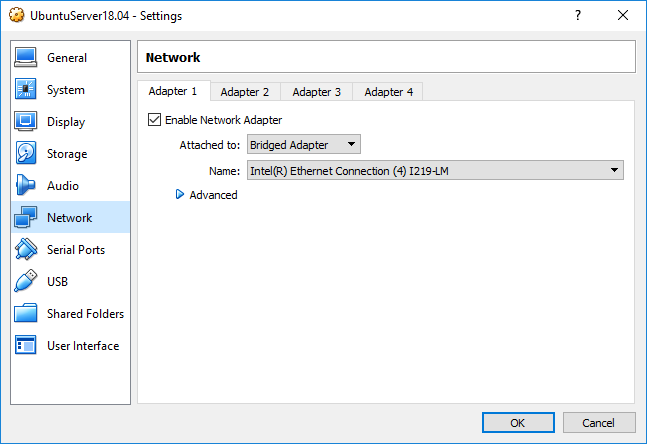
\includegraphics[scale=0.8]{VirtualBoxNetworkSettings}
	\caption{Oracle VM Virtual Box Network Settings}
	\label{fig:OracleVMSettings}
\end{figure}

You should have Matlab and Simulink installed.  Download the \textbf{matlab-sc1-model} folder from github\footnote{https://github.com/philippos-isaia/minicps} and load it into Matlab.  Open the model file in Simulink.  In the simulink window, press on the \textbf{Simulation} tab and choose \textbf{Pacing Options}.  \textbf{Enable} pacing in order to slow down the simulation.  This allows the simulation to run with near real-time behaviour.

Start the virtual machine that hosts miniCPS and run the scenario.  To run it, under the \textbf{minicps} directory run the command

\begin{lstlisting}[backgroundcolor = \color{ultralightgray}, language = Python, xleftmargin = 0.1cm, framexleftmargin = 0.3em, showstringspaces=false]
make matlab-sc1
\end{lstlisting}

\section{Description}
\label{cha:basicuse-sec:description}

As shown in Figure~\ref{fig:SimulinkModel} water flows from top to bottom (i.e. from~\textit{Tank 1} to~\textit{Tank (p1+s5)}).  Throughout its journey there are a number of sensors.  Sensors~\textit{s1} \&~\textit{s2} are pressure sensors, whereas sensors~\textit{s3} \&~\textit{s4} are flow sensors.  Sensor~\textit{s5} is a water level sensor that indicates the level of the water inside the Tank.
Finally~\textit{p2} is a centrifugal pump that is controlled from the remote emulated environment.


\begin{figure}[h!]
	\centering
	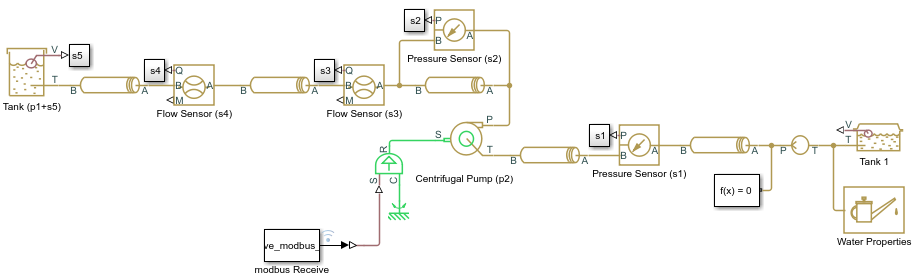
\includegraphics[scale=0.8, angle=90]{SimulinkScenario}
	\caption{Simulink Scenario Model}
	\label{fig:SimulinkModel}
\end{figure}


\section{Coordinator}
\label{cha:basicuse-sec:coordinator}

This version of miniCPS defines a new class called the~\textbf{Coordinator}.  This allows us to define the coordinator device which in Mininet is emulated as a typical switch.  

\begin{lstlisting}[backgroundcolor = \color{ultralightgray}, language = Python, xleftmargin = 0.1cm, framexleftmargin = 0.3em, showstringspaces=false]
class Coordinator(Device):

    """Coordinator class.
        Coordinator provides:
        - protocol server
        - communication with the DB
    """

    def __init__(
            self, name, protocol, state):
        """
        :param str name: device name
        :param dict protocol: used to set up 
                the network layer API
        :param dict state: used to set up 
                the physical layer API
        """

        super(Coordinator, self).
                __init__(name, protocol, state)
\end{lstlisting}

\noindent \\ In this particular example, the coordinator is initialised in~\textbf{first\_coordinator.py} which is then executed in switch~\textbf{s1}.

\noindent \\\textbf{TODO}: For now, the coordinator acts as a server that serves requests.  In the future we can add logic to the coordinator.


\section{PLCs}
\label{cha:basicuse-sec:plcs}


%\chapter{Extended Use}
%\label{cha:extendeduse}

\chapter{Docker}
\label{cha:docker}
\textbf{TODO} To be created after version 0.01 is evaluated and finalised

\begin{lstlisting}[backgroundcolor = \color{ultralightgray}, language = Python, xleftmargin = 0.1cm, framexleftmargin = 0.3em, showstringspaces=false]

\end{lstlisting}

\backmatter

\end{document}